\section{Auswertung}
\subsection{Bestimmung der Auflösung}
Aus dem aufgenommenen Spektrum der ThAr-Lampe kann empirisch eine Auflösung bestimmt werden, indem für mehrere Linien der Quotient aus Wellenlänge und Halbwertsbreite bestimmt und gemittelt wird. Dies wurde in MIDAS durchgeführt, indem über die Peaks eine Gaußfunktion gefittet wurde. Die erhaltenen Daten sind in Tabelle \ref{tab:Aufloesung}, Seite  \pageref{tab:Aufloesung} enthalten. Der Wert wurde also über die Formel
\begin{equation}
R_{Emp} = \frac{\lambda}{b}
\end{equation}
bestimmt, wobei $\lambda$ die Wellenlänge und $b$ die Halbwertsbreite ist. Der aus diesen Werten bestimmte Mittelwert mit Standardabweichung ergibt sich zu:
\begin{equation}
R_{Emp} = 13663.3 \pm 2445.8
\end{equation}
Dieser Wert lässt sich auch von MIDAS direkt berechnen, wobei MIDAS das Ergebnis
\begin{equation}
R_{Emp} = 12547.7 \pm 3398.3
\end{equation}
ausgibt. Es ist anzunehmen, dass MIDAS eine weitaus größere Anzahl von Linien für die Berechnung des Werts verwendet, deswegen ist dieser Wert trotz der größeren Standardabweichung als genauer anzunehmen.
\\
Es wurden bereits aus theoretischen Überlegungen Auflösungen für das Spektrometer und die CCD-Kamera bestimmt:
\begin{equation}
R_{Echelle} = 24416
\end{equation}
\begin{equation}
R_{CCD} =  25000
\end{equation}
Man sieht, dass die empirisch bestimmte Auflösung zwar in der gleichen Größenordnung, aber um ca. einen Faktor 2 kleiner ist.\
Dies ist vor allem dadurch begründet, dass die Kollimatorlinse nicht 'perfekt' ist, also verschiedene Wellenlängen unterschiedlich stark bricht. Dadurch verändert sich die Brennweite der Linse je nach Wellenlänge und das Bild wird unscharf. Eine Verbesserung der tatsächlichen Auflösung wäre also nur durch eine bessere, d.h. farbtreuere Linse möglich, dies würde aber die Kosten für den Spektrographen entsprechend hochtreiben.

\subsection{Auswertung der Spektren}
\subsubsection{Die Harvard-Klassifikation}
Die folgenden Informationen wurden entnommen aus \cite{ttunen}:\\
Sterne können anhand ihres Spektrums in verschiedene Typen eingeteilt werden. Diese Einteilung heißt Harvard-Klassifikation und ordnet Sterne in die Klassen O,B,A,F,G,K, oder M ein (fränkischer, geschlechtsneutraler Merkspruch: 'Ohne Bier ausm Fass gibts ka Maß'). Eine Einteilung der Sterne in diese Klassen ist anhand des Vorhandenseins bestimmter Absorptionslinien möglich. Der Unterschied zwischen Spektren von verschiedenen Sternen ist vor allem durch die Temperatur der Sterne bedingt. Die Linien werden durch Absorption von Photonen durch die Elektronen der Atome in der stellaren Atmosphäre erzeugt. So wird z.B. die Helium I - Linie durch Absorption von Photonen durch He-Atome im angeregten Zustand erzeugt. Der Übergang vom Grundzustand in den angeregten Zustand ist durch Photonen aus dem sichtbaren Spektrum nicht möglich. Um die He-Atome anzuregen, muss die Temperatur aber entsprechend hoch sein, sodass diese Linie in kalten Sternen nicht zu sehen ist. Bei höherer Temperatur sind auch mehr Atome im angeregten Zustand, womit mehr Photonen absorbiert werden und die Linie eine stärkere (bzw. niedrigere) Intensität erhält. Wenn die Temperatur weiter ansteigt, werden die He-Atome jedoch ionisiert und können daher keine Photonen mehr absorbieren, womit die Intensität der Linie wieder abnimmt (bzw. größer wird). Mit diesen Mechanismen lässt sich auch das Verhalten anderer Linien (Ca I, He II, Fe I) erklären. Bei Molekülen (z.B. TiO) gibt es so viele Übergänge, dass sie im Spektrum nicht mehr unterschieden werden können und als durchgängiges Absorptionsband erscheinen. Eine graphische Übersicht ist in Abb. \ref{fig:Harvard} dargestellt.
\\
Anhand der Absorptionslinien im Spektrum kann man nun einige Kriterien zur Einteilung angeben:
\begin{itemize}
\item Wenn das Spektrum nur wenige, dafür sehr intensive Linien zeigt, ist der Stern heiß, also in den Klassen O, B oder A.
\item Wenn das Spektrum sehr viele Linien zeigt, ist der Stern kalt, also in den Klassen F, G, K oder M.
\end{itemize}

Kalte Sterne zeigen viele Linien in ihrem Spektrum, da Elemente wie Eisen oder Calcium nur wenig Energie für die Übergänge zwischen Energieniveaus benötigen und aufgrund der großen Anzahl von Elektronen auch viele Übergänge besitzen. Bei heißen Sternen sind diese Atome bereits ionisiert und es dominieren die Übergänge von Wasserstoff und Helium.

\begin{table}
\centering
\begin{tabular}{c|c|c|c|c|c|c}

 & He II & He I & Fe II & Ca I & G-Band & TiO-Band \\ 
\hline 
O & $\bullet$ & $\bullet$ &  &  &  &  \\ 
\hline 
B &  & $\bullet$ &  &  &  &  \\ 
\hline 
A &  &  &  &  &  &  \\ 
\hline 
F &  &  & $\bullet$ &  &  & \\ 
\hline
G &  &  &  & $\bullet$ & $\bullet$ &  \\ 
\hline 
K &  &  &  & $\bullet$ &  &  \\ 
\hline 
M &  &  &  & $\bullet$ &  & $\bullet$ \\ 
\end{tabular}
\caption{Existenz von Absorptionslinien nach Spektralklasse}
\label{tab:Spektralklassen}
\end{table}

\begin{figure}
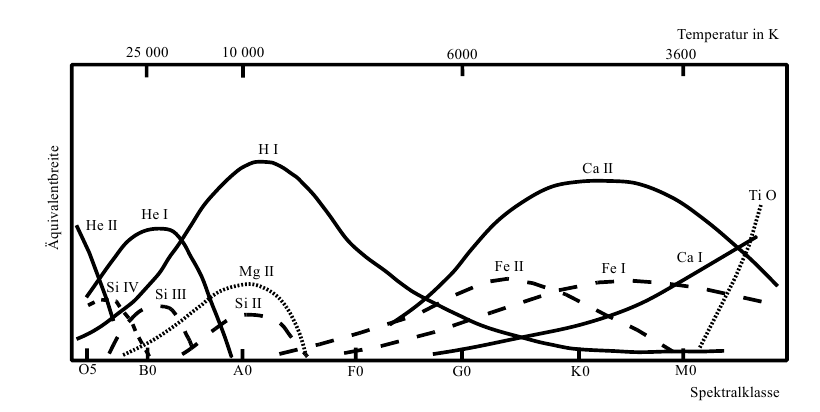
\includegraphics[width=1\textwidth]{images/Spektralklassen.png}
\caption{Qualitative Abhängigkeit der Äquivalentbreite einiger Elemente von der Spektralklasse/Temperatur eines Sternes (Abbildung entnommen aus \cite{ronomischesPraktikum})}
\label{fig:Harvard}
\end{figure}

Mit diesen beiden Kriterien und den in Tabelle \ref{tab:Spektralklassen} dargestellten Linien kann man Sterne sehr gut anhand ihres Spektrums in Spektraltypen einordnen. Da die Übergänge zwischen Spektraltypen fließend sind, ist die so gefundene Einordnung aber manchmal nicht eindeutig und es muss eine gründlichere Untersuchung durchgeführt werden, für die Zwecke des Praktikums ist dies aber ausreichend.

\subsubsection{Untersuchung des Sonnenspektrums}
In dem reduzierten aufgenommenen Sonnenspektrum wurden die wichtigsten Absorptionslinien (entnommen aus \cite{ronomischesPraktikum}) identifiziert und deren Position in MIDAS mittels einer gefitteten Gaußfunktion bestimmt. Die Abweichungen von den theoretischen Werten wurden bestimmt und daraus ein Mittelwert mit Standardabweichung berechnet. Die Werte sind in Tabelle \ref{tab:Sonne}, Seite \pageref{tab:Sonne} aufgetragen.\
Die Verschiebung von Spektrallinien ist durch den Dopplereffekt bedingt, der bei sich relativ zum Empfänger bewegenden Licht- bzw. allgemeinen Quellen auftritt. Da die Sonne jedoch relativ zur Erde keine Radialgeschwindigkeit besitzt, weil die Erde sich in einer Kreisbahn (Ellipsenbahn, dies ist hier aber vernachlässigbar,  da die Exzentrizität der Erdbahn sehr klein ist) um die Sonne bewegt, sollte keine Verschiebung auftreten.\
Aus den Daten wurde der Mittelwert und die Standardabweichung der Verschiebung zu
\begin{equation}
\overline{\Delta\lambda} = -0.021 \pm 0.086
\end{equation}
berechnet. Der Wert ist sehr klein und hat eine vergleichsweise große Standardabweichung. Er liegt damit im Bereich der Messgenauigkeit nahe des erwarteten Werts von 0, wobei hier natürlich eigentlich die elliptische Erdbahn mit einbezogen werden müsste. Für eine genauere Bestimmung des Werts müsste eine weitaus größere Zahl an Linien ausgewertet werden.
\\
\\
Weiterhin wurden im Sonnenspektrum und in den Spektren von zwei weiteren Sternen mit bekannter Klassifikation die Äquivalentbreiten von drei Linien mittels MIDAS bestimmt. Die Ergebnisse sind in Tabelle \ref{tab:Aequivalentbreite} eingetragen.

\begin{table}
\begin{center}
\begin{tabular}{c|c|c|c}
Stern & Linie & Wellenlänge in $\AA$ & Äquivalenzbreite \\ 
\hline 
Sonne & Ca I & 6122.23 & 0.203 \\ 
& Fe I & 6430.85 & 0.110 \\ 
& $H_\alpha$ & 6562.81 & 1.595 \\ 
\hline
$\sigma$ Dra & Ca I & 6122.23 & 0.310 \\ 
& Fe I & 6430.85 & 0.144 \\  
& $H_\alpha$ & 6562.81 & 1.401 \\ 
\hline
$\chi$ Dra & Ca I & 6122.23 & 0.148 \\ 
& Fe  I & 6430.85 & 0.049 \\ 
& $H_\alpha$ & 6562.81 & 1.632 \\ 
\end{tabular}
\caption{Messung der Äquivalentbreiten für die Sonne und die Sterne $\sigma$ Dra und $\chi$ Dra}
\label{tab:Aequivalentbreite}
\end{center}
\end{table} 

Aus Abb. \ref{fig:Harvard} ist zu erwarten, dass die Sonne als G-Stern für die Ca I-Linie eine kleinere Äquivalentbreite als der K-Stern $\sigma$ Dra aufweist, während die Ca I-Linie im F-Stern $\chi$ Dra fast nicht sichtbar sein sollte. Die Fe I-Linie sollte die größte Halbwertsbreite in $\sigma$ Dra aufweisen, die geringste in $\chi$ Dra. Die $H_\alpha$-Linie sollte die geringste Halbwertsbreite in $\sigma$ Dra, die größte Halbwertsbreite in $\chi$ Dra aufweisen.\
Diese Vermutungen werden durch die Messdaten im Wesentlichen bestätigt, wobei noch erwähnt werden sollte, dass der Wert für die Ca I-Linie im F-Stern $\chi$ Dra doch relativ groß ist. Dies liegt daran, dass $\chi$ Dra ein 'später', also kalter F-Stern (F7) ist, und deswegen noch genügend nicht ionisierte Ca-Atome vorliegen.
\subsubsection{Untersuchung des Sternspektrums}
Das aufgenommene und reduzierte Sternspektrum wurde mit einem Spektralatlanten verglichen, um es mit Hilfe der vorher beschriebenen Kriterien in die Harvard-Klassifikation einordnen zu können. Dies wurde ebenfalls für zwei andere Sternspektren (ab sofort 'Stern 2' und 'Stern 3' genannt) durchgeführt.
\paragraph{Beobachteter Stern}
\begin{figure}
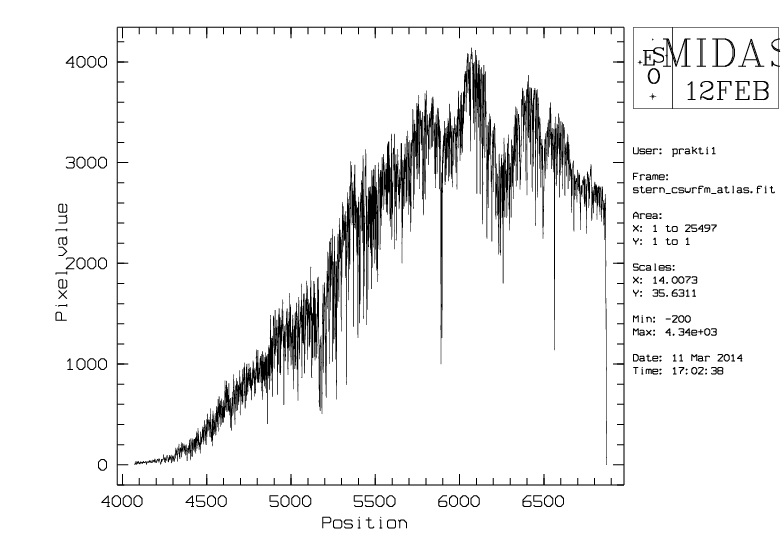
\includegraphics[height=.4\textheight]{images/stern_messung_spektrum.png}
\caption{Spektrum des beobachteten Sterns}
\label{fig:stern_messung_spektrum}
\end{figure}
In Abbildung \ref{fig:stern_messung_spektrum}, Seite \pageref{fig:stern_messung_spektrum} ist das Spektrum des beobachteten Sterns dargestellt. Es sind viele Linien zu erkennen, weswegen zu vermuten ist, dass der Stern zu den kalten Spektralklassen F,G,K und M gehört.
\\
\begin{figure}
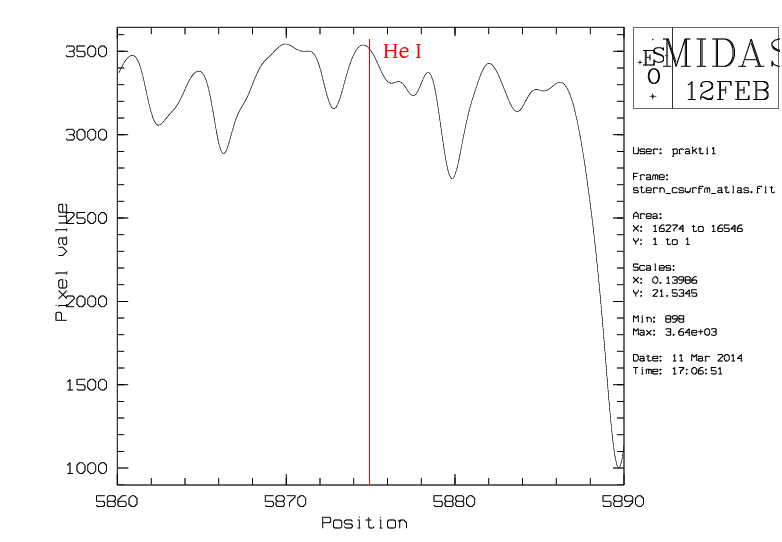
\includegraphics[height=.4\textheight]{images/stern_messung_HeI.png}
\caption{Mögliche Position der HeI-Linie im Spektrum des beobachteten Sterns}
\label{fig:stern_messung_HeI}
\end{figure}
Wie in Abbildung \ref{fig:stern_messung_HeI}, Seite \pageref{fig:stern_messung_HeI} zu erkennen, ist im Spektrum des beobachteten Sterns keine He I-Linie bei $5875.70 \AA$ identifizierbar, ein weiteres Indiz dafür, dass der Stern zu den kalten Spektralklassen gehört.
\\
\begin{figure}
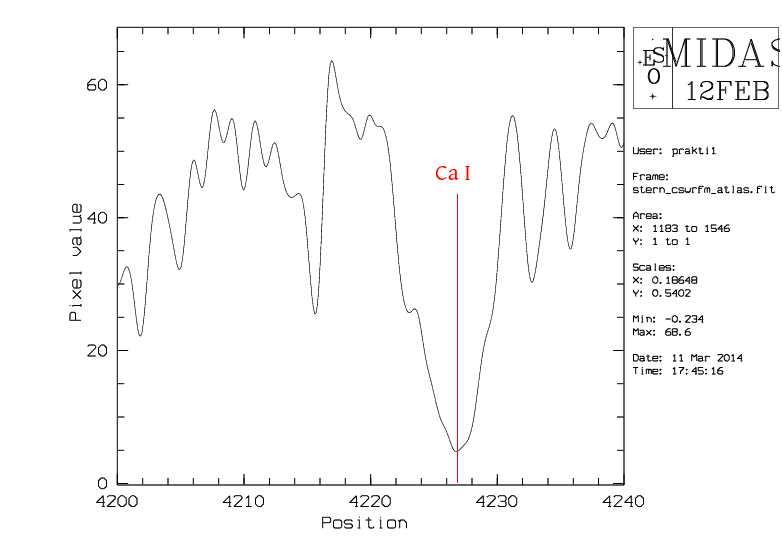
\includegraphics[height=.4\textheight]{images/stern_messung_CaI.png}
\caption{Position der CaI-Linie im Spektrum des beobachteten Sterns}
\label{fig:stern_messung_CaI}
\end{figure}
In Abbildung \ref{fig:stern_messung_CaI}, Seite \pageref{fig:stern_messung_CaI} ist die CaI-Linie bei $4226.74 \AA$ klar identifizierbar, also ist der Stern wahrscheinlich nicht in Klasse F.
\\
\begin{figure}
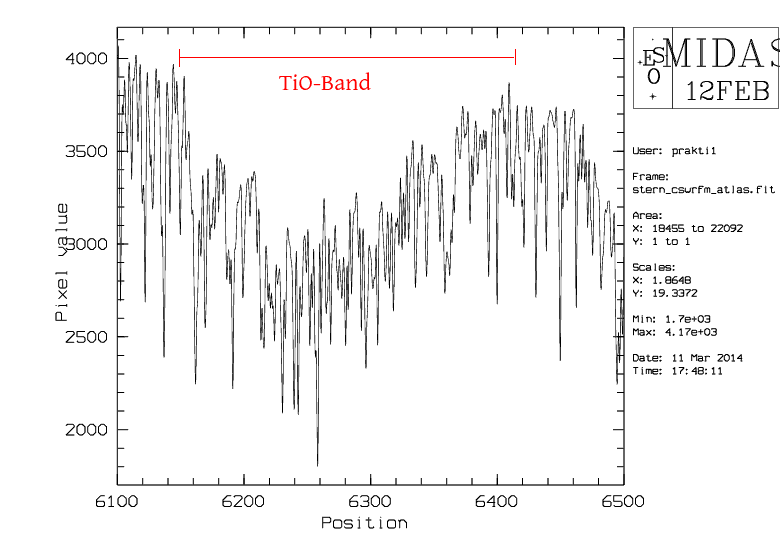
\includegraphics[height=.4\textheight]{images/stern_messung_TiO.png}
\caption{Position des TiO-Bands im Spektrum des beobachteten Sterns}
\label{fig:stern_messung_TiO}
\end{figure}
In Abbildung \ref{fig:stern_messung_TiO}, Seite \pageref{fig:stern_messung_TiO} ist das TiO-Band zwischen den Wellenlängen $6200 - 6400 \AA$ gut zu erkennen, welches nur in Klasse M-Sternen vorkommt.\
\\
Diese Indizien sprechen klar dafür, dass der beobachtete Stern in die Spektralklasse M einzuordnen ist.

\paragraph{Stern 2}
\begin{figure}
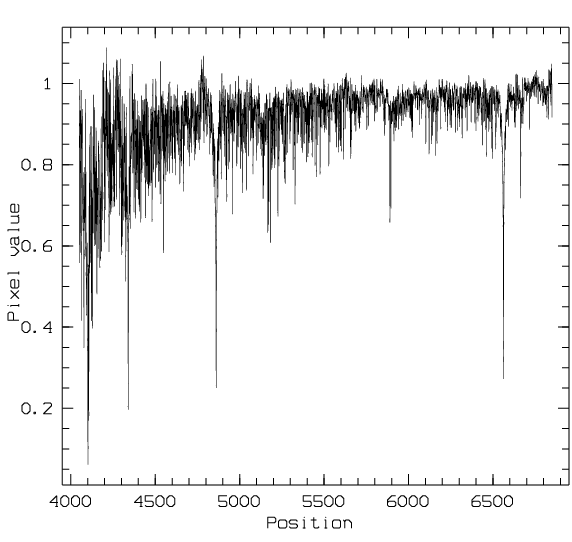
\includegraphics[height=.4\textheight]{images/stern2_spektrum.png}
\caption{Spektrum von Stern 2}
\label{fig:stern2_spektrum}
\end{figure}
Im Spektrum von Stern 2 (Abbildung \ref{fig:stern2_spektrum}, Seite \pageref{fig:stern2_spektrum}) sind viele Linien zu erkennen, was wiederum darauf schließen lässt, dass der Stern in die Klassen F,G,K oder M einzuordnen ist.
\\
\begin{figure}
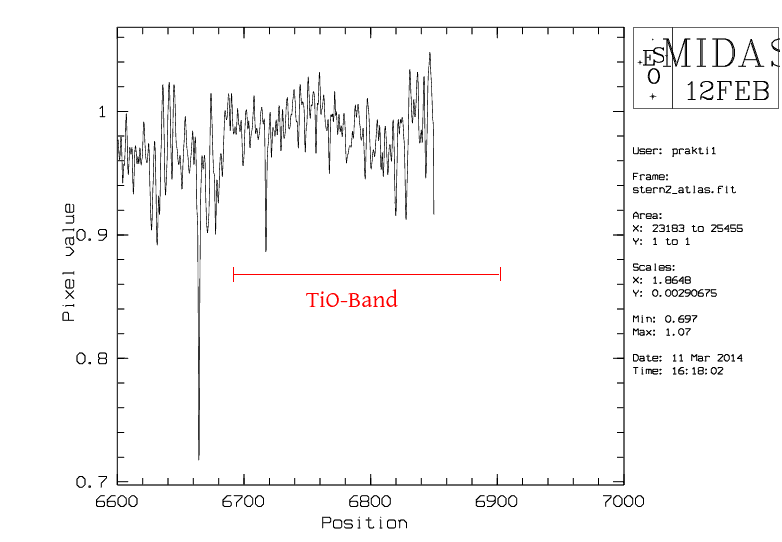
\includegraphics[height=.4\textheight]{images/stern2_TiO.png}
\caption{Mögliche Position des TiO-Bandes im Spektrum von Stern 2}
\label{fig:stern2_TiO}
\end{figure}
Zwischen den Wellenlängen $6700-7000 \AA$ ist kein TiO-Band zu erkennen, was eine Einteilung in Klasse M ausschließt.
\\
\begin{figure}
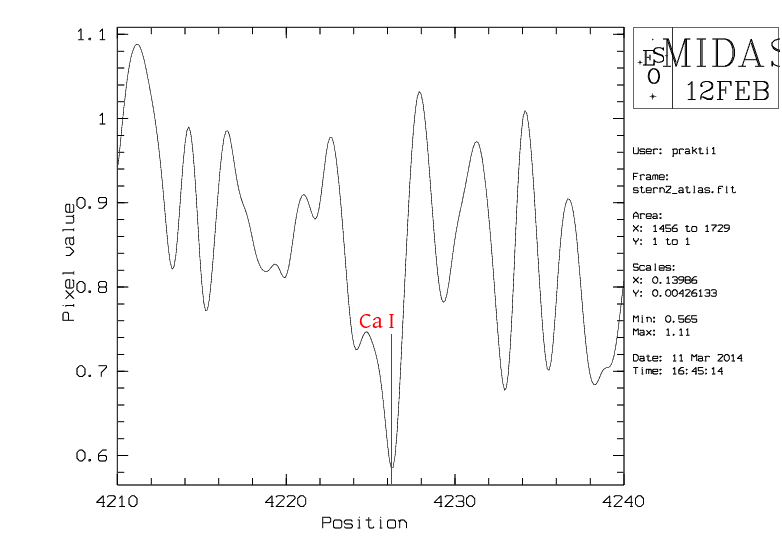
\includegraphics[height=.4\textheight]{images/stern2_CaI.png}
\caption{Position der CaI-Linie im Spektrum von Stern 2}
\label{fig:stern2_CaI}
\end{figure}
Bei der Wellenlänge $4226.74 \AA$ ist die CaI-Linie klar identifizierbar, weswegen der Stern nicht in die Klasse F eingeordnet werden kann.
\\
\begin{figure}
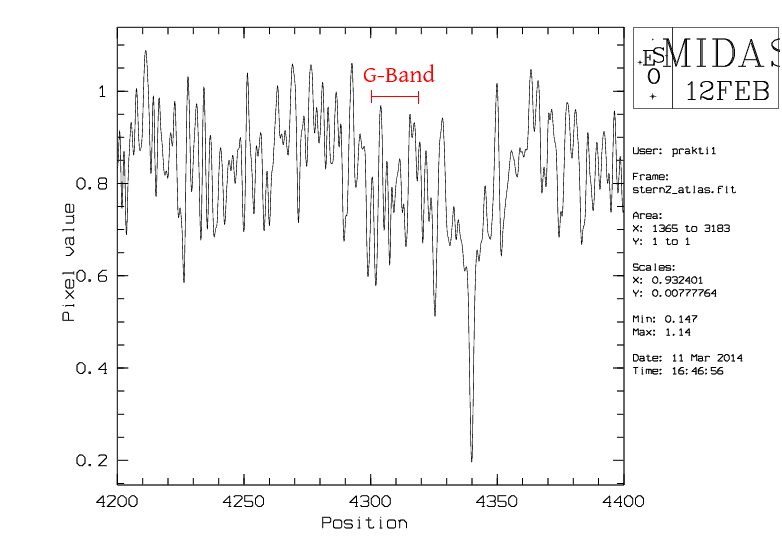
\includegraphics[height=.4\textheight]{images/stern2_G-Band.png}
\caption{Mögliche Position des G-Bandes im Spektrum von Stern 2}
\label{fig:stern2_CaI}
\end{figure}
In der Umgebung der Wellenlänge $4310 \AA$ ist kein G-Band zu erkennen, weshalb der Stern kein G-Stern sein kann.
\\
Damit bleibt nur noch die Klasse K als mögliche Einteilung übrig.

\paragraph{Stern 3}
\begin{figure}
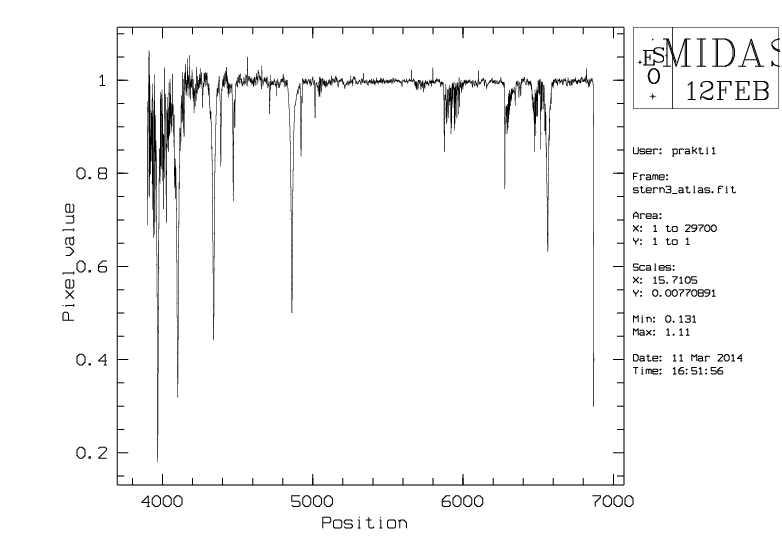
\includegraphics[height=.4\textheight]{images/stern3_spektrum.png}
\caption{Spektrum von Stern 3}
\label{fig:stern3_spektrum}
\end{figure}
Im Spektrum von Stern 3 (Abbildung \ref{fig:stern3_spektrum}, Seite \pageref{fig:stern3_spektrum}) sind wenige Linien mit einigen klar definierten Peaks zu erkennen. Daraus lässt sich schließen, dass der Stern in die heißen Spektralklassen O,B oder A  eingeordnet werden muss.

\begin{figure}
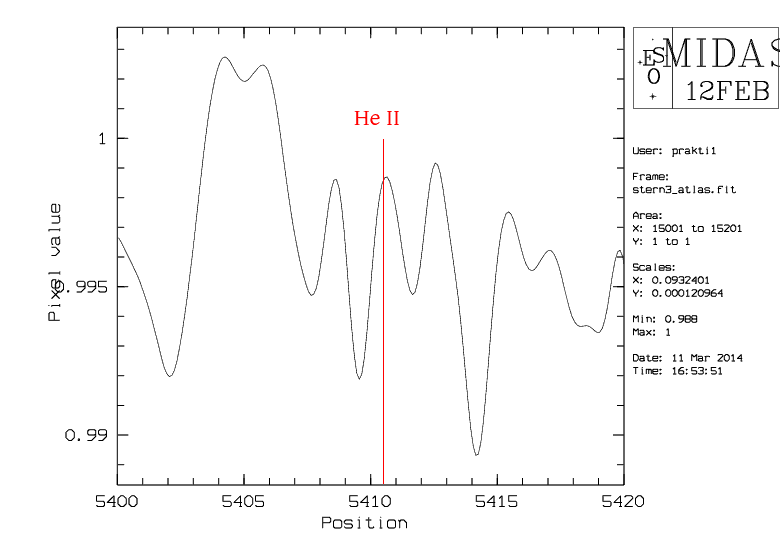
\includegraphics[height=.4\textheight]{images/stern3_HeII.png}
\caption{Mögliche Position der HeII-Linie im Spektrum von Stern 3}
\label{fig:stern3_HeII}
\end{figure}
Bei $5411.52 \AA$ ist keine HeII-Linie identifizierbar, der Stern kann also kein O-Stern sein.
\\
\begin{figure}
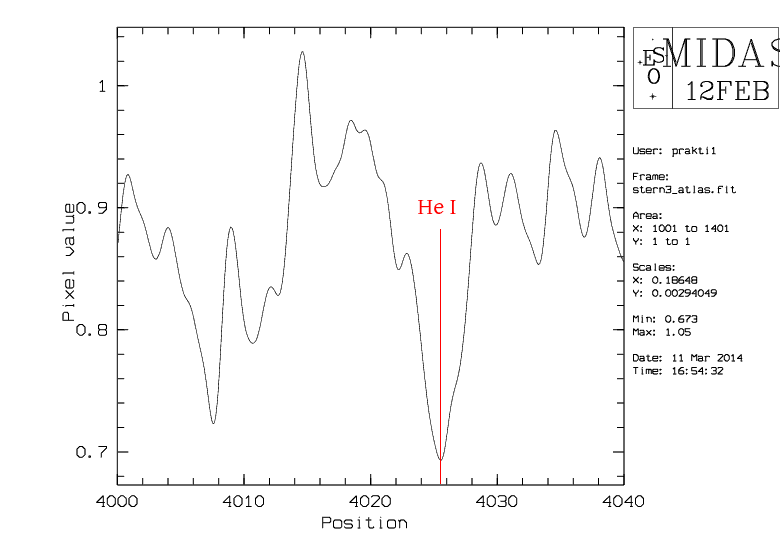
\includegraphics[height=.4\textheight]{images/stern3_HeI.png}
\caption{Position der HeI-Linie im Spektrum von Stern 3}
\label{fig:stern3_HeI}
\end{figure}
Die HeI-Linie bei $4026.20 \AA$ ist eindeutig erkennbar. Daraus lässt sich nun schließen, dass der Stern innerhalb der Spektralklasse B einzuordnen ist.

\newpage
\subsubsection{Bestimmung der Radialgeschwindigkeit}
Im Spektrum des gemessenen Sterns wurden mehrere Linien identifiziert und mit den theoretischen Wellenlängen verglichen, um die Dopplerverschiebung zu bestimmen. Hierbei sind alleinstehende und schmale Linien zu bevorzugen, weil sich durch die Verschiebung sonst Linien überlagern könnten.\
Die Geschwindigkeiten wurden mit der relativistischen Dopplerformel (die klassische Formel wäre auch ausreichend gewesen, hat jedoch zunächst absurde Ergebnisse geliefert, was evtl. an fehlerhafter Eingabe im Rechner lag)
\begin{equation}
f_B = f_Q \sqrt{\frac{c+v}{c-v}} \Leftrightarrow v = \frac{f_B^2 - f_Q^2}{f_B^2 + f_Q^2} \cdot c = \frac{\lambda_Q^2 - \lambda_B^2}{\lambda_B^2 + \lambda_Q^2}\cdot c
\end{equation}
wobei die Größen mit Index B für den Betrachter und Q für die Quelle stehen.\
Die Ergebnisse sind in Tabelle \ref{tab:Radial} dargestellt.

\begin{table}[htbp]
\begin{tabular}{c|c|c|c|c}
Element & theoretische Wellenlänge in $\AA$ & gemessene Wellenlänge in $\AA$ & $\Delta\lambda$ & V in km/s \\ \hline
Ca I & 4226.74 & 4226.685 & 0.055 & 3.90 \\ 
Fe I & 4383.56 & 4383.705 & -0.145 & -9.92 \\ 
Fe I & 5328.05 & 5328.087 & -0.037 & -2.10 \\ 
Ca I & 6162.18 & 6161.736 & 0.444 & 21.60 \\ 
Na I & 5889.97 & 5889.672 & 0.298 & 15.17 \\ 
Fe I & 4891.5 & 4890.983 & 0.517 & 31.70 \\ 
\end{tabular}
\caption{Bestimmung von Radialgeschwindigkeiten für den gemessenen Stern}
\label{tab:Radial}
\end{table}

Aus den berechneten Geschwindigkeiten lässt sich ein Mittelwert mit Standardabweichung berechnen, dies ist aber aus mehreren Gründen nicht sonderlich aussagekräftig. Der berechnete Wert wäre
\begin{equation}
\overline{v} = 10.1 \pm 15.6 \ \mathrm{km/s}
\end{equation}
Die Standardabweichung ist offensichtlich sehr groß, was vor allem daran liegt, dass nur wenige Linien ausgewertet wurden und der Fit in MIDAS auch nur begrenzte Genauigkeit hat. Vor allem treten sowohl positive als auch negative Verschiebungen auf, weswegen aus diesen Ergebnissen keine klare Erkenntnis gewonnen werden kann. 
Weiterhin muss gesagt werden, dass die Verschiebung sich aus mehreren Komponenten zusammensetzt, so bewegt sich nicht nur der Stern radial von der Erde weg, sondern auch die Sternwarte wegen der Erddrehung, die Erde bewegt sich um die Sonne, das Sonnensystem um das galaktische Zentrum und die Milchstraße relativ zur Galaxie des Sterns. Die Bestimmung der Geschwindigkeit des Sterns relativ zur Erde ist also nicht so einfach durchzuführen. 


